\appendix

\section{Formal Definitions of Baseline Samplers}
\label{appendix:baselines}

To provide a rigorous comparison, we formalize the action selection mechanism for each baseline sampler. At each decoding step $t$, let $p_\theta(\cdot \mid z_t, \ell)$ denote the predicted token distribution at masked position $\ell \in \mathcal{M}_t$. The samplers differ in their scoring function $\phi(z_t, \ell)$, where the top-$K$ positions with the lowest scores are selected for decoding.

\paragraph{Uniform~\cite{nie2025large}} This baseline selects positions uniformly at random from the mask set $\mathcal{M}_t$:
\begin{equation}
    \phi_{\text{Uniform}}(z_t, \ell) = \epsilon, \quad \epsilon \sim \mathcal{U}(0, 1)
\end{equation}

\paragraph{Confidence~\cite{chang2022maskgit}} This baseline prioritizes positions where the model is most certain about the top-1 prediction:
\begin{equation}
    \phi_{\text{Conf}}(z_t, \ell) = \max_{v \in \mathcal{V}} p_\theta(v \mid z_t, \ell)
\end{equation}

\paragraph{Entropy~\cite{ye2025dream}} Positions with the minimum predictive uncertainty are selected:
\begin{equation}
    \phi_{\text{neg entropy}}(z_t, \ell) = \sum_{v \in \mathcal{V}} p_\theta(v \mid z_t, \ell) \log p_\theta(v \mid z_t, \ell)
\end{equation}

\paragraph{Margin~\cite{kim2025train}} This baseline considers the gap between the two most likely tokens, selecting positions with the largest margin:
\begin{equation}
    \phi_{\text{Margin}}(z_t, \ell) = p_{\text{top1}} - p_{\text{top2}}
\end{equation}

\paragraph{KLASS~\cite{kim2025klass}} This method incorporates a KL-divergence constraint to maintain consistency between consecutive decoding steps. Originally, KLASS~\cite{kim2025klass} supports dynamic decoding by selecting all positions that satisfy the KL threshold. To ensure a fair performance comparison with other samplers, we adapt it to decode a fixed number of tokens per step. Following the original implementation, we set the threshold $\epsilon = 5 \times 10^{-4}$. Effectively, KLASS prioritizes positions where the KL divergence is below the threshold, ranking them by confidence, and only falls back to other positions if more tokens are required. This can be formalized as the following scoring function:
\begin{equation}
    \phi_{\text{Conf}}(z_t, \ell)+\textbf{1}_{(D_{KL}(p_\theta(\cdot \mid z_t, \ell) \| p_\theta(\cdot \mid z_{t+1}, \ell)) < \epsilon)} \\
\end{equation}
where positions with higher scores are prioritized. In our experiments, we first select positions satisfying the KL constraint based on confidence, and then fill the remaining budget from the other positions.

\paragraph{PC-Sampler~\cite{huang2025pc}} This sampler regulates the decoding trajectory by combining a position-aware weight with content-aware confidence calibration. It modulates the selection priority of each candidate token $x_\ell$ at position $\ell$ using an exponential decay function $w_\ell = e^{-\lambda \cdot \ell}$, where $\lambda \ge 0$ controls the positional penalty. To discourage generic tokens, it calibrates the confidence score using the token frequency distribution $p_{\mathcal{D}'}(x_\ell)$ and a content-aware calibration term $\mathcal{C}^{(\ell)
}_t$:
\begin{equation}
    \phi_{\text{PC}}(z_t, \ell) = \mathcal{C}^{(\ell)
}_t \cdot w_\ell
\end{equation}

\paragraph{Block Diffusion~\cite{arriola2025block,wu2025fast}} This sampler employs a position scheduling function $I_t(\ell)$ that indicates whether position $\ell$ lies within the currently active diffusion block at time step $t$. Specifically, $I_t(\ell)$ takes the value 1 if $\ell \in \mathcal{B}_{\sigma(t)}$ and 0 otherwise, where $\mathcal{B}_{\sigma(t)}$ denotes the active block determined by a scheduling rule $\sigma(t)$. The sampling process restricts candidate positions to the active block and applies a standard heuristic:
\begin{equation}
\phi_{\text{Block}}(z_t, \ell) = 
\begin{cases} 
\phi(z_t, \ell), & \text{if } I_t(\ell) = 1, \\
-\infty, & \text{otherwise}.
\end{cases}
\end{equation}
Here, the active block $\mathcal{B}_{\sigma(t)}$ slides over time according to $\sigma(t)$, typically following a sequential or random traversal of the position indices, thereby gradually diffusing information across the entire sequence.


\paragraph{LookUM~\cite{lee2025lookahead}}
This framework improves decoding in masked diffusion language models by selecting optimal token unmasking orders during inference. Unlike myopic heuristics that consider only immediate next steps, LookUM generates multiple candidate unmasking trajectories (paths) and selects the most promising one based on global sequence-level certainty. This can be formalized as the following scoring function:
\begin{equation}
    \phi_{\text{LookUM}}(z_t, \ell) = \frac{1}{|M_{t-1}|} \cdot\sum_{\ell \in M_{t-1}}\phi(z_{t-1}, \ell)
\end{equation}
where $M_{t-1}$ denotes the set of masked positions at the previous timestep, and $\phi(\cdot)$ is a base metric that can be instantiated as negative entropy, confidence, or margin. Following the empirical findings in the paper~\cite{lee2025lookahead}, we adopt negative entropy as our specific implementation of $\phi(\cdot)$ due to its demonstrated effectiveness in capturing sequence-level uncertainty. We omit the design of SMC and NIS in LookUM~\cite{lee2025lookahead} to enable a clear comparison, as they require task-specific parameter tuning.
neiji
\section{Detailed Hyperparameter Settings}
\label{appendix:hyperparameters}

In this section, we provide a detailed overview of the hyperparameter settings used across all experiments. All experiments were conducted on NVIDIA A800 GPUs.

\noindent\textbf{Reasoning and Coding Tasks.} For tasks involving logical reasoning (GSM8K, MATH500) and code generation (HumanEval, MBPP), we set the token sampling temperature $\tau_{\text{token}} = 0.7$ to strike a balance between output diversity and structural coherence. For the Info-Gain Sampler, we employ a relatively low position temperature $\tau_{\text{pos}} = 0.1$ to focus the selection on the most informative candidate positions, while generating $N=8$ candidate actions per step for parallel evaluation. To maintain high throughput during predictable decoding phases, we set the acceleration threshold $\gamma = 0.8$, which allows the sampler to skip the full evaluation routine when the maximum token probability is high. For block diffusion settings on Semi-AR models (SDAR and TraDo), we use a fixed block size of 16. The decoding budget $K$ (tokens per step) is varied between 1 and 2 to evaluate performance under different acceleration ratios. Maximum generation lengths are benchmark-specific: 256 tokens for GSM8K, HumanEval, and MBPP; 512 tokens for MATH500 and SDAR benchmarks; and 1024 tokens for the TraDo-8B model to accommodate longer reasoning chains.

\noindent\textbf{Text-to-Image Generation.} For multimodal experiments using the MMaDa model on ImageNet and GenEval, we adopt a more conservative token temperature $\tau_{\text{token}} = 0.4$ and a matching position temperature $\tau_{\text{pos}} = 0.4$ to ensure high fidelity and alignment with text prompts. The candidate set size is kept at $N=8$. We follow a 50-step decoding trajectory governed by a cosine schedule, which progressively reduces the number of masked positions to refine image details. For extreme acceleration tests (Section~\ref{appendix:few_step}), we utilize a 5-step linear schedule to evaluate the sampler's robustness under severe budget constraints.

\noindent\textbf{Creative Writing.} We evaluate creative writing performance using 200 prompts selected from the Alpaca dataset. Following the Min-P paper~\cite{nguyen2024turning}, we employ GPT-4.1~\cite{openai_gpt4_1} as an LLM judge to assess generation quality. For this experiment, the maximum generation length is set to 1024 tokens, with a fixed block size of 16.

% \noindent\textbf{Baselines} All baseline samplers (Uniform, Confidence, Entropy, Margin, KLASS, and PC-Sampler) are configured with the same token temperature $\tau_{\text{token}}$ as our method to ensure a fair comparison. For KLASS, we set the consistency threshold $\epsilon = 5 \times 10^{-4}$ following its original implementation. For PC-Sampler, we adopt the default decay parameters for positional weighting as specified in the original work.






\section{Theoretical Analysis of the Info-Gain Objective}
\label{appendix:mi_upper_bound}



\paragraph{Setup and notation.}
At decoding step $t$, let $z_t$ denote the current state and $\mathcal{M}_t$ the set of masked positions.  
For each $\ell \in \mathcal{M}_t$, define the per-position predictive entropy
\begin{equation}
H^{(\ell)}(z_t) := H\big(X^{(\ell)} \mid z_t\big),
\end{equation}
and the average state uncertainty
\begin{equation}
\mathcal{H}(z_t) := \frac{1}{|\mathcal{M}_t|} \sum_{\ell \in \mathcal{M}_t} H^{(\ell)}(z_t).
\end{equation}

For an action $a_t$ selecting positions $A_t \subseteq \mathcal{M}_t$, the next state is $z_{t-1} = \mathrm{Apply}(z_t, a_t)$ and $\mathcal{M}_{t-1} = \mathcal{M}_t \setminus A_t$. The Info-Gain objective is defined as
\begin{equation}
\mathrm{IG}(a_t; z_t) := \mathcal{H}(z_t) - \mathcal{H}(z_{t-1}), \qquad
C(a_t \mid z_t) := \sum_{\ell \in A_t} H^{(\ell)}(z_t),
\end{equation}
\begin{equation}
J_{\mathrm{IG}}(a_t; z_t) := C(a_t \mid z_t) - \mathrm{IG}(a_t; z_t),
\end{equation}
where $C(a_t\mid z_t)$ measures the immediate uncertainty of the chosen positions, and $\mathrm{IG}(a_t; z_t)$ quantifies the reduction in overall state uncertainty.

\paragraph{Expected information gain.}
Sampling $a_t$ from a sampler $\pi(\cdot \mid z_t)$ induces randomness in $\mathrm{IG}(a_t; z_t)$ and $J_{\mathrm{IG}}(a_t; z_t)$. Let
\begin{equation}
\tilde{I}(A_t; z_t) := \mathbb{E}[\mathrm{IG}(a_t; z_t)], \qquad
J_{MI}(A_t; z_t) := \mathbb{E}[J_{\mathrm{IG}}(a_t; z_t)],
\end{equation}
where the expectation is over the sampled token assignments while keeping $A_t$ fixed.

\begin{observationbox}
\begin{proposition}[Upper bound on expected information gain]
\label{prop:mibound}
For any state $z_t$ and position set $A_t \subseteq \mathcal{M}_t$,
\begin{equation}
\tilde{I}(A_t; z_t) \le C(a_t \mid z_t), \qquad \text{and thus} \quad J_{MI}(A_t; z_t) \ge 0.
\end{equation}
\end{proposition}
\end{observationbox}

\begin{proof}
Define
\begin{equation}
\alpha := \frac{1}{|A_t|} \sum_{\ell \in A_t} H^{(\ell)}(z_t), \quad
\beta := \frac{1}{|\mathcal{M}_{t-1}|} \sum_{\ell \in \mathcal{M}_{t-1}} H^{(\ell)}(z_t), \quad
\gamma := \frac{|A_t|}{|\mathcal{M}_t|}.
\end{equation}
Then $C(a_t \mid z_t) = |A_t| \alpha$ and $\mathcal{H}(z_t) = \gamma \alpha + (1-\gamma) \beta$.

Let $Y := X^{(A_t)}$ be the sampled assignments. For any $\ell \in \mathcal{M}_{t-1}$,
\begin{equation}
I(Y; X^{(\ell)} \mid z_t) \le \min(H(Y\mid z_t), H^{(\ell)}(z_t)) \le \min(|A_t| \alpha, H^{(\ell)}(z_t)).
\end{equation}
By the entropy-reduction decomposition,
\begin{equation}
\tilde{I}(A_t; z_t) = \gamma (\alpha - \beta) + \frac{1}{|\mathcal{M}_{t-1}|} \sum_{\ell \in \mathcal{M}_{t-1}} \mathbb{E}[I(Y; X^{(\ell)} \mid z_t)].
\end{equation}

\noindent \textbf{Case 1:} $\alpha \le \beta$. Then $I(Y; X^{(\ell)} \mid z_t) \le |A_t| \alpha$, giving
\begin{equation}
\tilde{I}(A_t; z_t) \le \gamma (\alpha - \beta) + |A_t| \alpha \le |A_t| \alpha = C(a_t \mid z_t).
\end{equation}

\noindent \textbf{Case 2:} $\alpha > \beta$. Then $I(Y; X^{(\ell)} \mid z_t) \le H^{(\ell)}(z_t)$ and
\begin{equation}
\tilde{I}(A_t; z_t) \le \gamma (\alpha - \beta) + \beta \le \alpha \le |A_t| \alpha = C(a_t \mid z_t).
\end{equation}

In both cases, $\tilde{I}(A_t; z_t) \le C(a_t \mid z_t)$, implying
\begin{equation}
J_{MI}(A_t; z_t) = C(a_t \mid z_t) - \tilde{I}(A_t; z_t) \ge 0.
\end{equation}
\end{proof}
\paragraph{Practical implications.}
Proposition~\ref{prop:mibound} establishes that, for any fixed position set $A_t$, the expected Info-Gain objective $J_{MI}(A_t; z_t)$ is non-negative. This provides a theoretical guarantee that, on average, the cost of committing to selected positions is never underestimated relative to the actual reduction in state uncertainty. In practice, we find that the realized $J_{\mathrm{IG}}(a_t; z_t)$, computed along individual decoding trajectories, closely tracks this expectation. On benchmarks such as GSM8K, more than $95\%$ of observed $J_{\mathrm{IG}}$ values are non-negative or slightly below zero (e.g., $J_{\mathrm{IG}} \ge -5\times 10^{-4}$), indicating that the bound is rarely violated. 

Furthermore, $\mathrm{IG}(a_t; z_t)$ is highly semantically sensitive: it captures not only the immediate uncertainty of the chosen positions but also how these assignments influence the uncertainty of the remaining masked positions. As a result, $J_{\mathrm{IG}}(a_t; z_t)$ naturally discourages actions that would commit to poorly conditioned or inconsistent states, effectively preventing error propagation during decoding. This behavior manifests as a strong implicit correction mechanism, enabling the sampler to recover from suboptimal early decisions and maintain coherent, high-quality generation. Overall, the Info-Gain objective provides a computationally efficient and robust signal for action selection, balancing immediate certainty with long-term state stability throughout the iterative decoding process.

\begin{figure}[t]
    \centering
    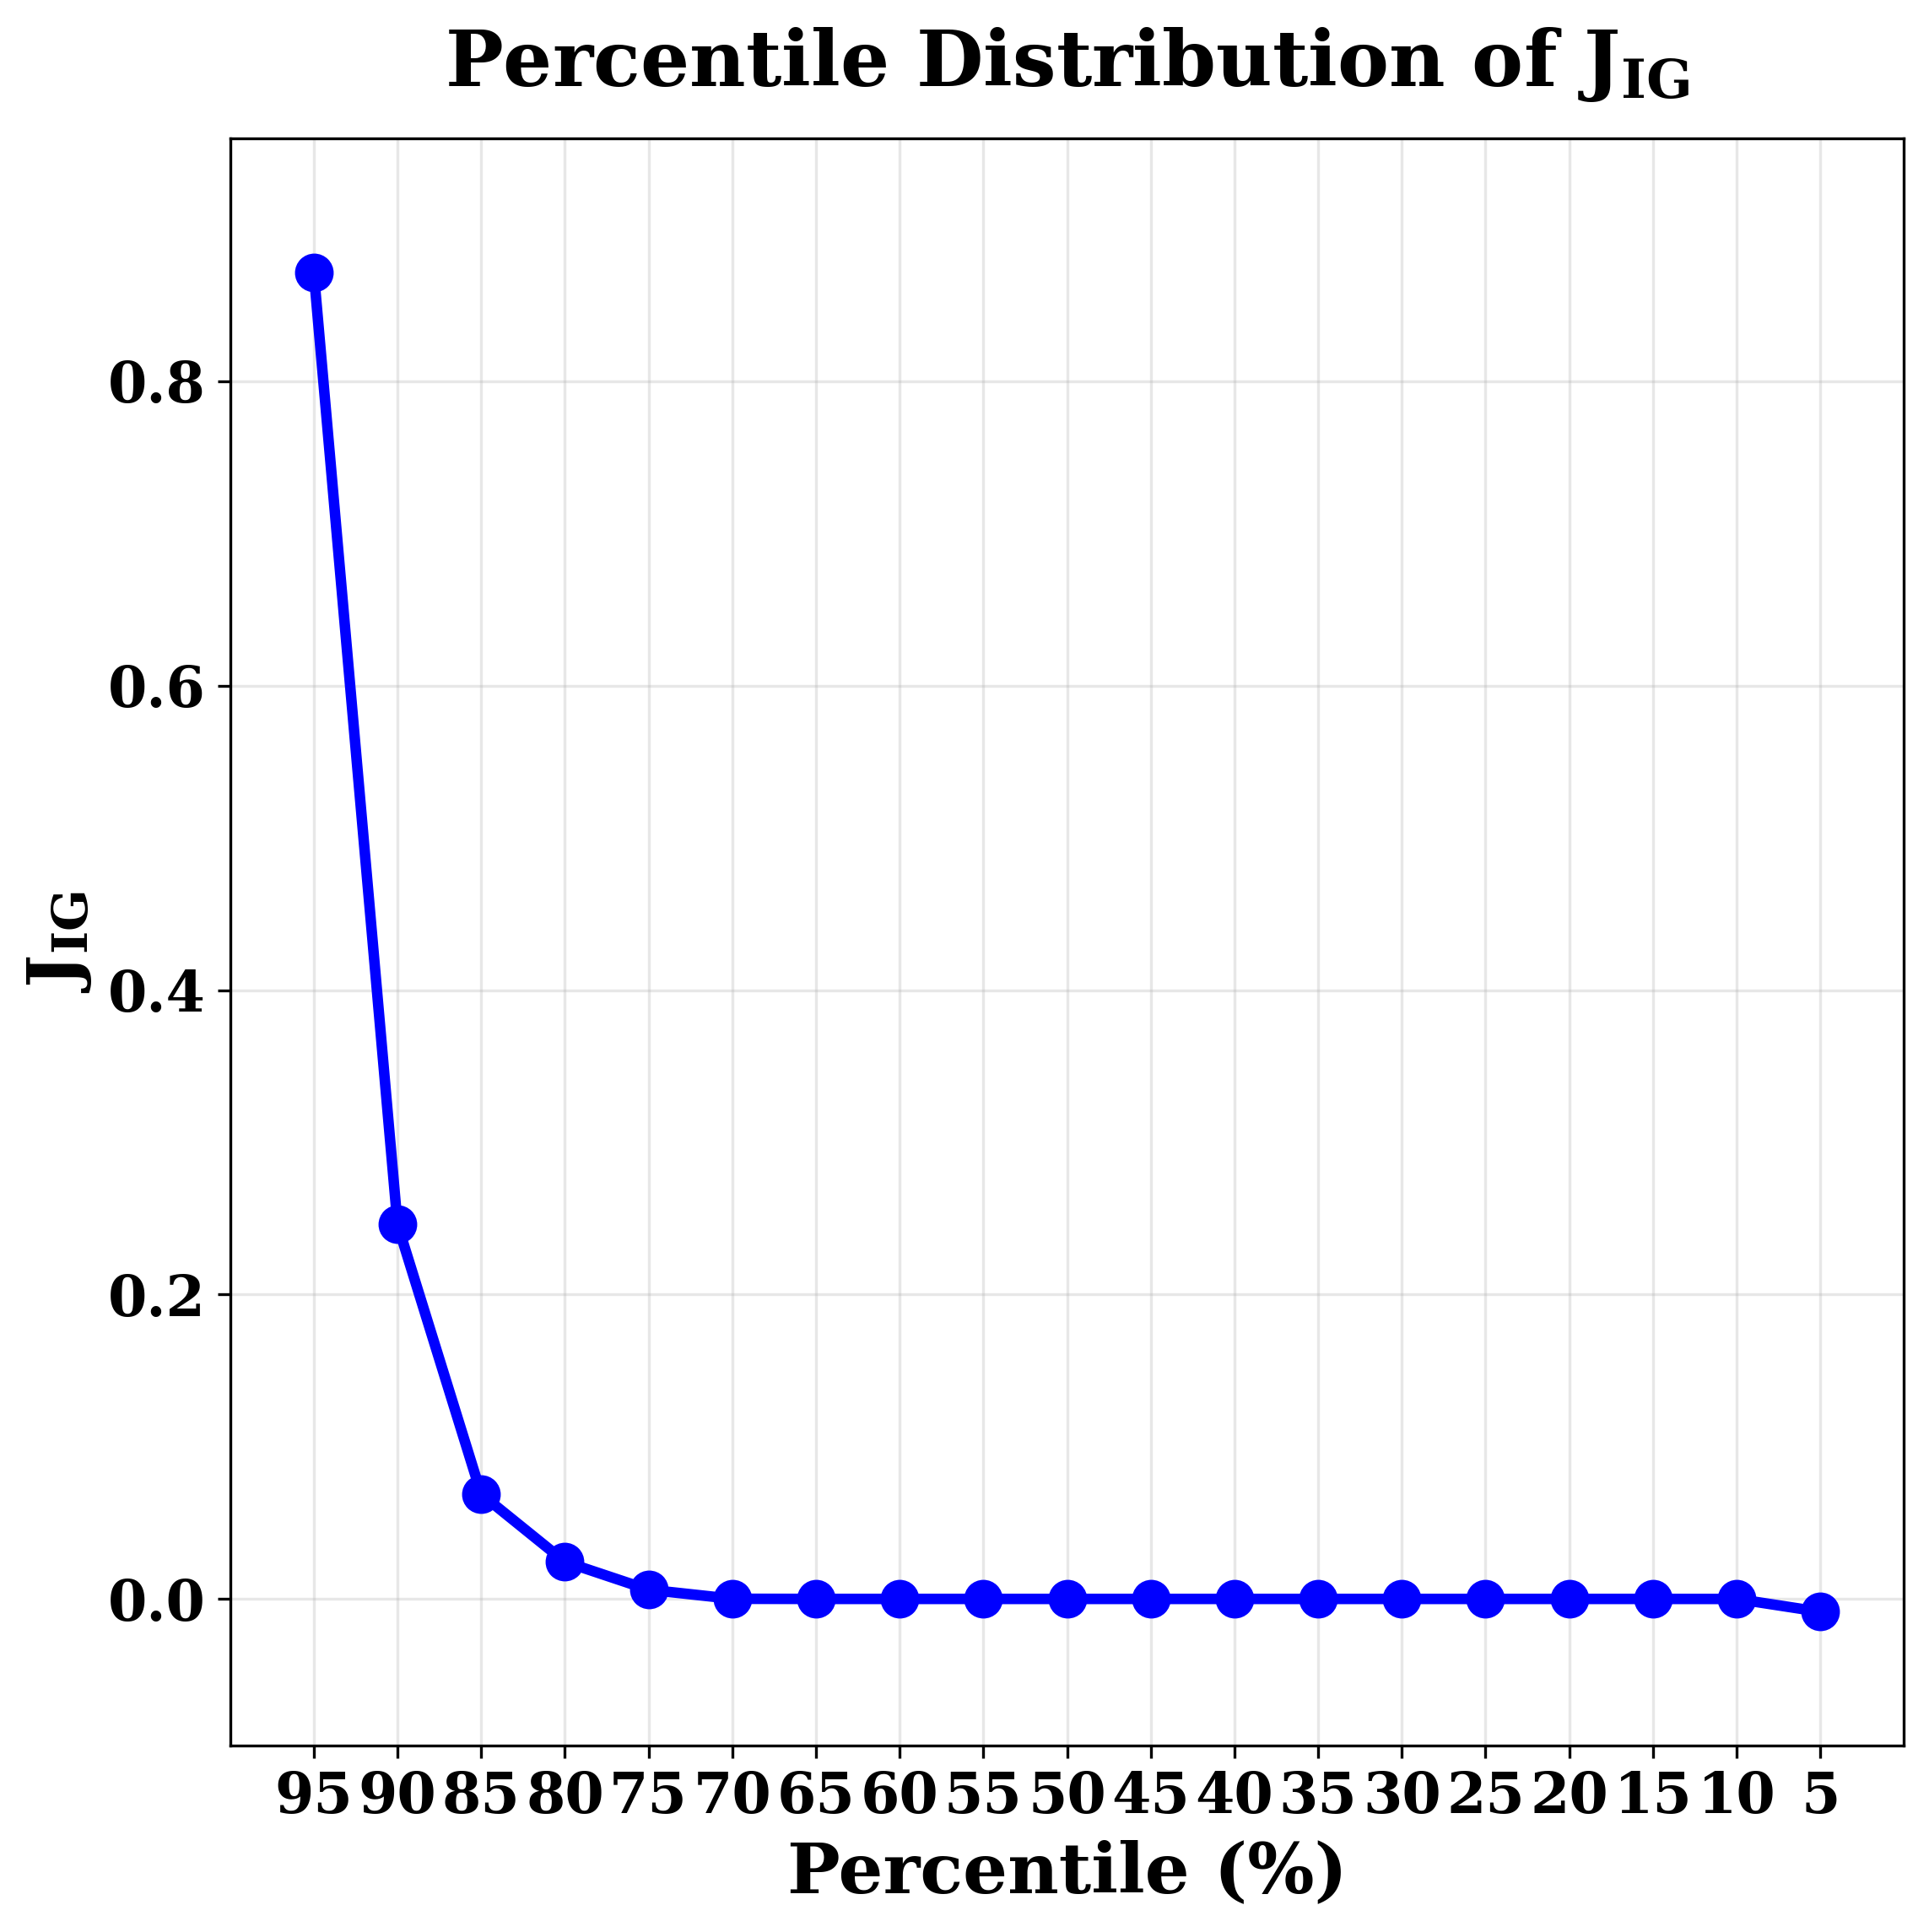
\includegraphics[width=0.5\linewidth]{bound.png}
    \caption{Empirical distribution of $J_{IG}$ values sorted from highest to lowest. The 5th percentile is $-5 \times 10^{-4}$, indicating the bound is rarely violated in practice.}
    \label{fig:jig_distribution}
\end{figure}


\section{Pseudo codes for Info-Gain Sampler and Info-Gain Beam Search}
\label{appendix:pseudo-code}
We provide PyTorch-style pseudo codes for the implementation of Info-Gain Sampler and Info-Gain Beam Search.




\subsection{Info-Gain Sampler}
\begin{lstlisting}[style=pytorch, caption={Info-Gain Sampler}]
def info_gain_sampler(model, seq_len, K, N):
    # Initialize: all positions masked
    z = torch.full((1, seq_len), MASK_ID)
    
    # Initial forward pass
    with torch.no_grad():
        logits = model(z)  # [1, seq_len, vocab_size]
    
    for t in range(K):
        # 1. Sample candidate actions
        candidates = action_sampler(z, model, N) 
        
       # 2. Parallel Evaluation
        z_candidates = apply(z,candidates)
        logits_candidates = model(z_candidates)
        costs = compute_information_gain(logits,logits_candidates)
        
        # 3. State Transition
        best_idx = torch.argmin(costs)
        z = z_candidates[best_idx:best_idx+1]
        logits = logits_candidates[best_idx:best_idx+1]
    return z
\end{lstlisting}
\subsection{Info-Gain Beam Search}
\begin{lstlisting}[style=pytorch, caption={Info-Gain Beam Search}, label={alg:igp_beam}]
def ig_beam(model, seq_len, K, N, beam_size):
    # Initialize the queue
    beam = [(torch.full((1, seq_len), MASK_ID), 0.0)]
    
    for t in range(K):
        next_beam_candidates = []
        next_f = []
        
        # Expand each beam
        for z, g in beam:
            # 1. Action Sampling
            candidates = action_sampler(z, model, num_candidates=N)
            
            # 2. Update Beam candidates
            z_candidates = apply(z, candidates)
            logits_candidates = model(z_candidates)
            transition_costs = compute_cost(candidates)
            state_values = compute_state(logits_candidates)
            
            g_candidates = g + transition_costs
            f_candidates = g_candidates + state_values
            
            for i in range(N):
                next_beam_candidates.append((z_candidates[i:i+1], g_candidates[i]))
                next_f.append(f_candidates[i])
        
        # 3. Selection
        f_tensor = torch.tensor(next_f)
        kept_indices = torch.argsort(f_tensor)[:beam_size] 
        beam = [next_beam_candidates[i] for i in kept_indices]
    
    beam.sort(key=lambda x: x[1])
    best_z, best_g = beam[0]
    return best_z
\end{lstlisting}

\section{Experiments in Extremely Low-Step Generation Scenarios}
\label{appendix:few_step}

In this section, we present additional experimental results for scenarios where the number of decoding steps is severely constrained.

First, we present the results for the ImageNet-512 benchmark using the MMaDa model in a text-to-image generation setting. The experimental configuration is similar to that in Section~\ref{sec:exp}, with the key difference being the use of a linear step schedule and a highly constrained budget of only 5 decoding steps. As shown in Figure~\ref{fig:imagenet512_extreme_steps}, our method demonstrates significantly better visual quality and structural coherence under these extreme conditions. Furthermore, we visualize the evolution of cumulative entropy averaged over 10,000 sampled instances in Figure~\ref{fig:geneval_entropy_evolution}.
\begin{figure*}[h]
    \centering
    \begin{subfigure}{0.4\linewidth}
        \centering
        
\includegraphics[width=\linewidth]{IGS.png}
        \caption{Info-Gain}
    \end{subfigure}
    \hspace{1em}
    \begin{subfigure}{0.4\linewidth}
        \centering
        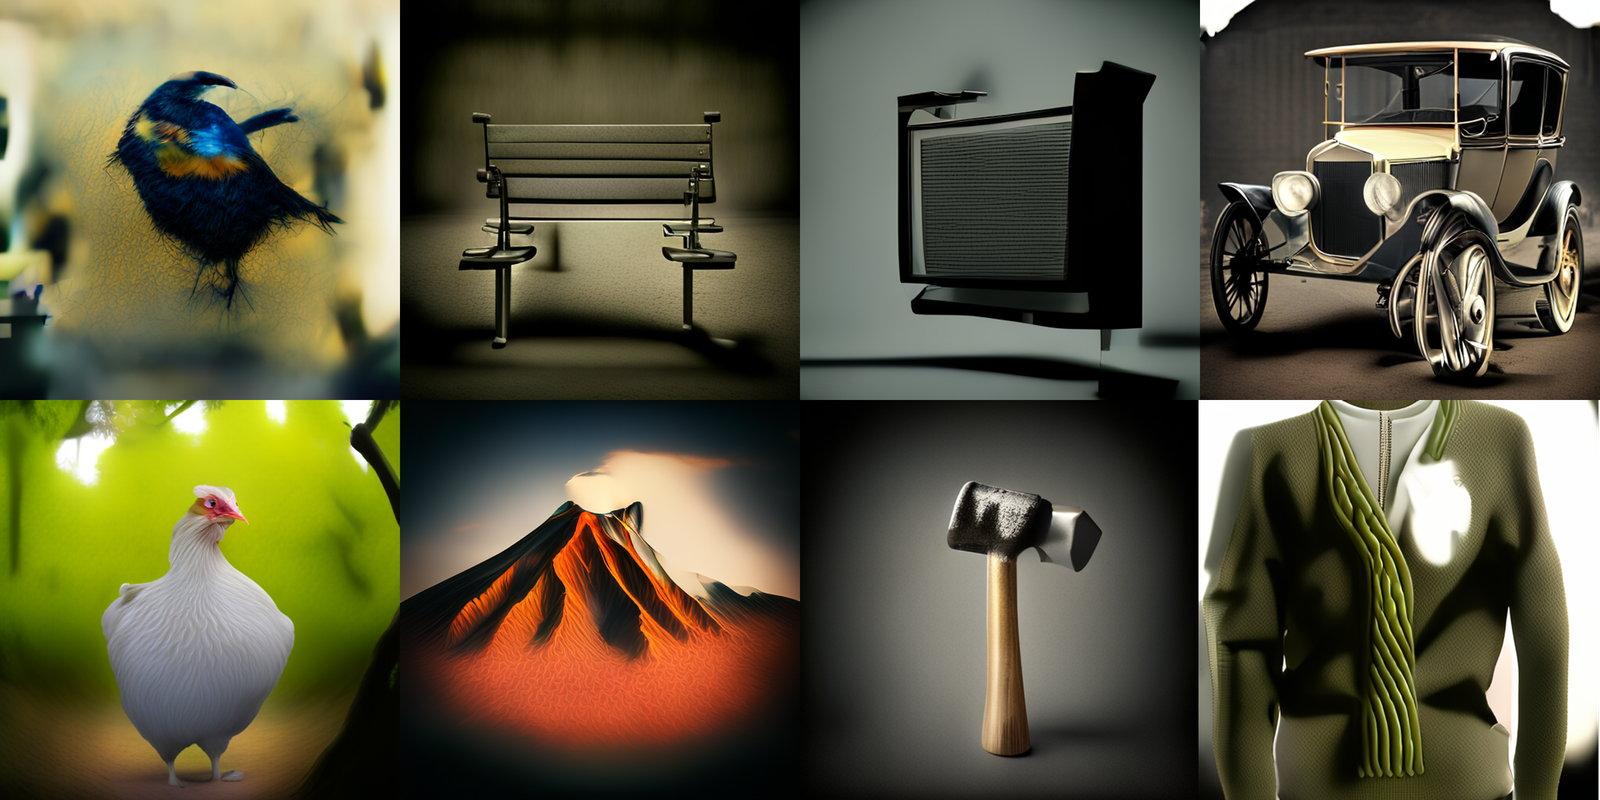
\includegraphics[width=\linewidth]{Confidence.png}
        \caption{Confidence}
    \end{subfigure}
    
    \vspace{1em}
    
    \begin{subfigure}{0.4\linewidth}
        \centering
        \includegraphics[width=\linewidth]{entropy.png}
        \caption{Entropy}
    \end{subfigure}
    \hspace{1em}
    \begin{subfigure}{0.4\linewidth}
        \centering
        
\includegraphics[width=\linewidth]{margin.png}
        \caption{Margin}
    \end{subfigure}
    \caption{Visual results on ImageNet-512 with an extreme budget of only 5 decoding steps. The Info-Gain Sampler maintains superior structural coherence compared to baseline heuristics.}
    \label{fig:imagenet512_extreme_steps}
\end{figure*}

\begin{figure}
    \centering
    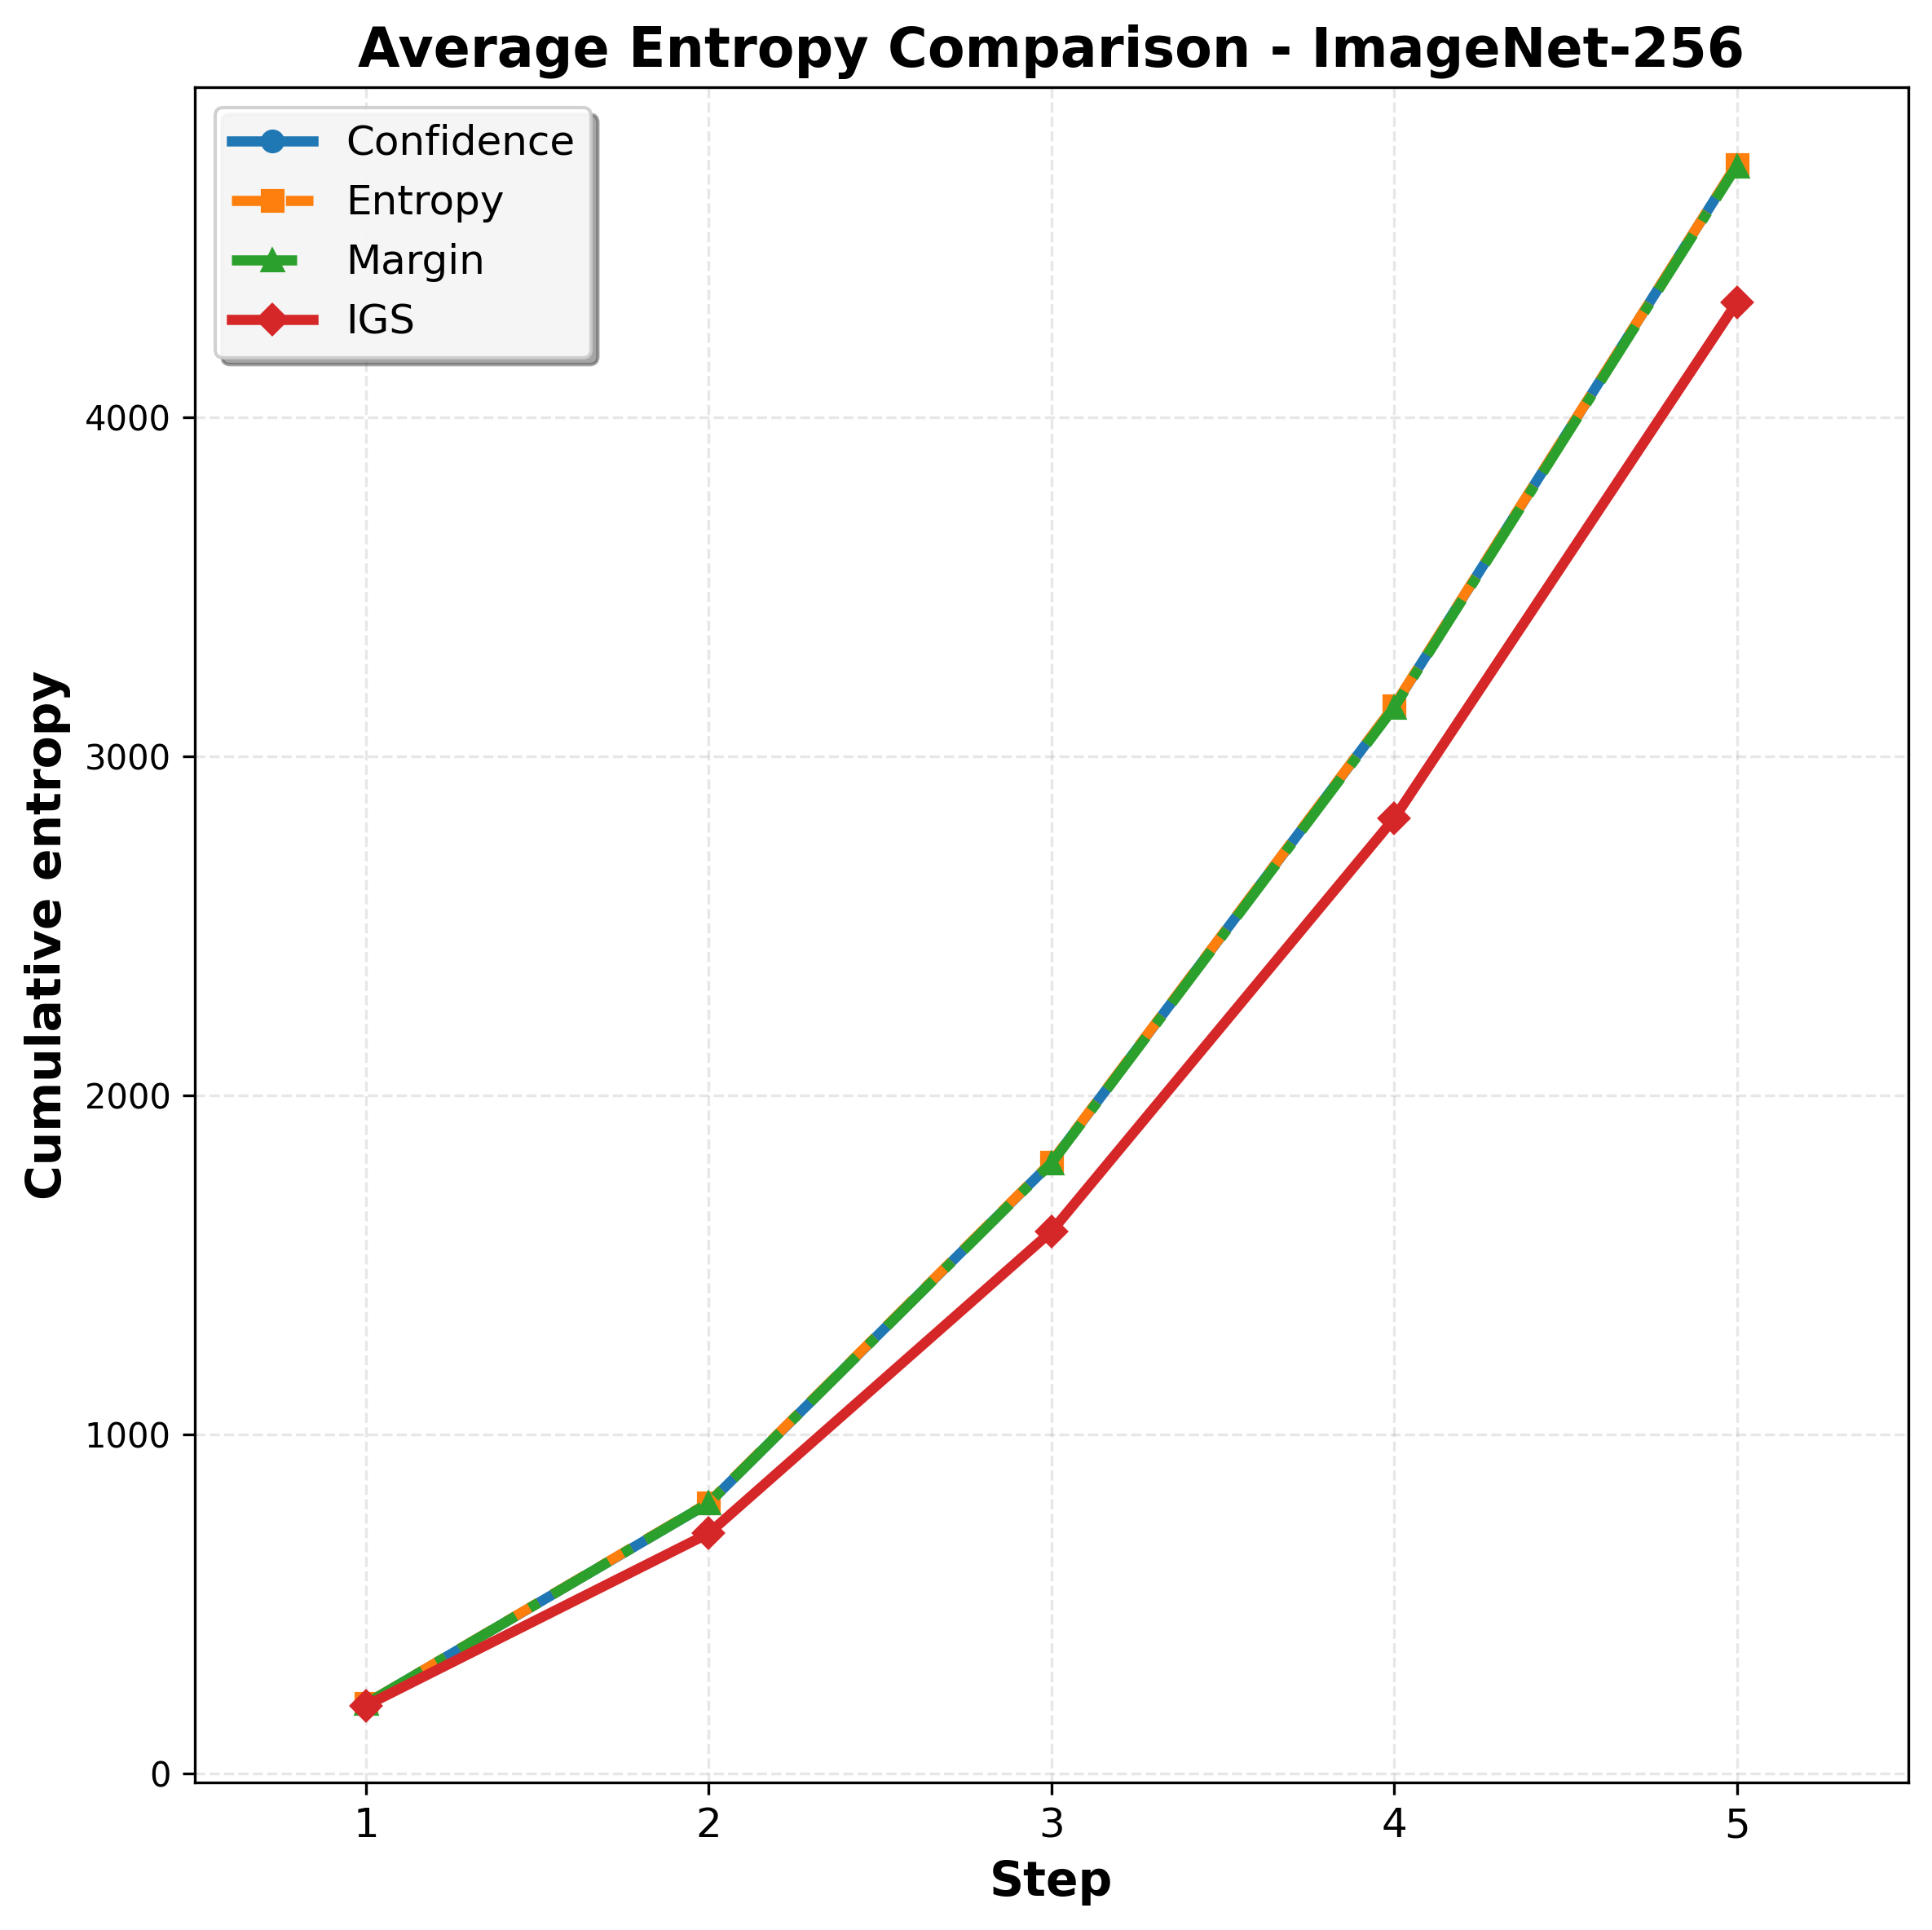
\includegraphics[width=0.5\linewidth]{imagenet256-compare.png}
    \caption{Evolution of cumulative entropy during image generation on the Image256 benchmark. The results are averaged over all labels using a 5-step linear schedule. The curves illustrate how Info-Gain Sampler manages global uncertainty compared to other methods throughout the decoding process.}
    \label{fig:geneval_entropy_evolution}
\end{figure}




To further evaluate the robustness of our sampler, we conduct an ultra-low step generation experiment using the Dream Model. We construct a simple writing task containing 50 prompts (e.g., ``Write a story about a cat'') and require the model to decode the content within a very small number of steps, for a fixed length of 80 tokens. In this extreme regime, most baselines fail to generate meaningful and coherent text. We record the "Collapse Step" for each method, defined as the minimum number of steps required to ensure that fewer than 50\% of the generated samples exhibit severe repetitions or grammatical errors.

For all experiments, the token sampling temperature is set to 0.4. For Info-Gain Sampler, the position sampling temperature is 0.4 and the number of action sets is $N=8$. The results are summarized in Table~\ref{tab:collapse_steps}.

\begin{table}[ht]
    \centering
    \caption{Comparison of Collapse Steps on ultra-low step writing tasks. Lower values indicate better robustness in extreme acceleration scenarios.}
    \label{tab:collapse_steps}
    \begin{tabular}{lc}
        \toprule
        Sampler & Collapse Step ($\downarrow$) \\
        \midrule
        Entropy & 13 \\
        Confidence & 12 \\
        Margin & 12 \\
        \textbf{Info-Gain} & \textbf{8} \\
        \bottomrule
    \end{tabular}
\end{table}

The purpose of both experiments in ultra-low step generation is to evaluate how to generate meaningful content under conditions of extremely limited information and few decoding steps. The performance of the greedy sampler is significantly inferior to that of the Info-Gain Sampler. This demonstrates that by balancing the utilization of immediate information with the information gain for future decisions, the Info-Gain Sampler effectively achieves the most meaningful generation within a restricted number of decoding steps.


\section{Resource Overhead Analysis}
\subsection{Memory Overhead Analysis}
\label{appendix:memory}

Let $M_W$ denote model weights, $M_A$ activations, and $M_C(L)$ the KV-cache for sequence length $L$. The key difference lies in how memory scales with the number of candidates $N$:



\begin{enumerate}
    \item \textbf{Non-cached Inference:} $M_{\text{total}} = M_W + N \cdot M_A$
    \item \textbf{Info-Gain Sampler (Shared Prefix):} $M_{\text{total}} = M_W + M_C(L-1) + N \cdot M_A$
    \item \textbf{Info-Gain Beam Search (Diverse Prefixes):} $M_{\text{total}} = M_W + N \cdot M_C(L-1) + N \cdot M_A$
\end{enumerate}

For Info-Gain Sampler, the additional memory cost for increasing $N$ is dominated by transient activations $M_A$, which are relatively small compared to weights $M_W$. In contrast, Info-Gain Beam Search requires storing $N$ separate KV-caches $M_C(L-1)$, leading to linear memory explosion with $N$. This is shown in Table~\ref{tab:memory_comparison_summary}

\begin{table}[h]
\centering
\caption{Memory efficiency comparison under KV-caching.}
\label{tab:memory_comparison_summary}
\resizebox{\columnwidth}{!}{
\begin{tabular}{lcc}
\toprule
\textbf{Method} & \textbf{KV-Cache Count} & \textbf{Memory Scaling} \\ \midrule
Info-Gain Sampler & 1 (shared) & $O(M_W + M_C + N \cdot M_A)$ \\
Info-Gain Beam Search & $B$ (diverse) & $O(M_W + B \cdot M_C + N\cdot B \cdot M_A)$ \\ \bottomrule
\end{tabular}}
\end{table}

Empirical measurements on TraDo-8B-Instruct (512 tokens, block size 16) validate this analysis. As shown in Figure~\ref{fig:gpu-compare}, Info-Gain Sampler maintains stable memory usage with only 24\% overhead at $N=8$, while Info-Gain Beam Search exhibits substantial memory surge due to divergent trajectory caching.
\subsection{Computation Overhead Analysis}
\label{appendix:computation}

The computational overhead of Info-Gain Sampler stems primarily from evaluating $N$ candidates per step. The theoretical time complexity is:
\begin{equation}
T_{\text{theoretical}} = K \cdot N \cdot T_f
\label{eq:complexity}
\end{equation}
where $K$ is decoding steps, $N$ is candidates per step, and $T_f$ is one forward pass cost.

\textbf{Practical optimizations significantly reduce overhead:}
\begin{enumerate}
    \item \textbf{Batched Parallel Evaluation:} All $N$ candidates are processed simultaneously:
    \begin{equation}
    T_{\text{batch}} = K \cdot (T_f + \epsilon), \quad \epsilon \ll (N-1)T_f
    \end{equation}
    
    \item \textbf{KV-Cache Reuse:} Shared prefix reduces attention computation:
    \begin{equation}
    T_{\text{cached}} \approx K \cdot T_{\text{prefix}} + \frac{K(N-1)}{N} T_{\text{attn}}
    \end{equation}
    
    \item \textbf{High-confidence Bypass:} If the maximum token probability exceeds a threshold $\gamma$, the full sampling routine is skipped to reduce latency.
\end{enumerate}

% \begin{table}[h]
% \centering
% \small
% \caption{Average time comparison (seconds) on reasoning tasks across different models and settings.}
% \label{tab:time_comparison}
% \begin{tabular}{@{}llcc@{}}
% \toprule
% \textbf{Model} & \textbf{Setting} & \textbf{Baselines} & \textbf{Info-Gain} \\
% \midrule
% Dream-7B & $K=2$ ($N=8$) & 9.7--13.3 & 18.4 (+64$\pm$26\%) \\
% & $K=1$ ($N=8$) & 20.6--24.0 & 25.5 (+15$\pm$9\%) \\
% \midrule
% SDAR-8B & $K=1$ ($N=8$) & 8.7--11.1 & 14.1 (+45$\pm$18\%) \\
% TraDo-8B & $K=1$ ($N=8$) & 12.0--12.4 & 17.3 (+42$\pm$2\%) \\
% \bottomrule
% \end{tabular}
% \end{table}

As shown in Fig.~\ref{fig:threshold_tradeoff}, our adaptive threshold mechanism effectively manages computational cost while maintaining high decoding quality. By dynamically adjusting the candidate acceptance threshold, we achieve near-optimal entropy reduction with minimal time overhead. This explains why practical speedups (1.2–1.5$\times$) are significantly better than theoretical predictions ($N\times$). While evaluating more candidates ($N$) increases per-step cost, it often reduces total steps ($K$) needed for convergence. Our batched implementation and threshold optimization ensure that the quality improvements are achieved with only a modest increase in overhead (typically 20–40\% on average for reasoning tasks).

\begin{figure*}[h]
    \centering
    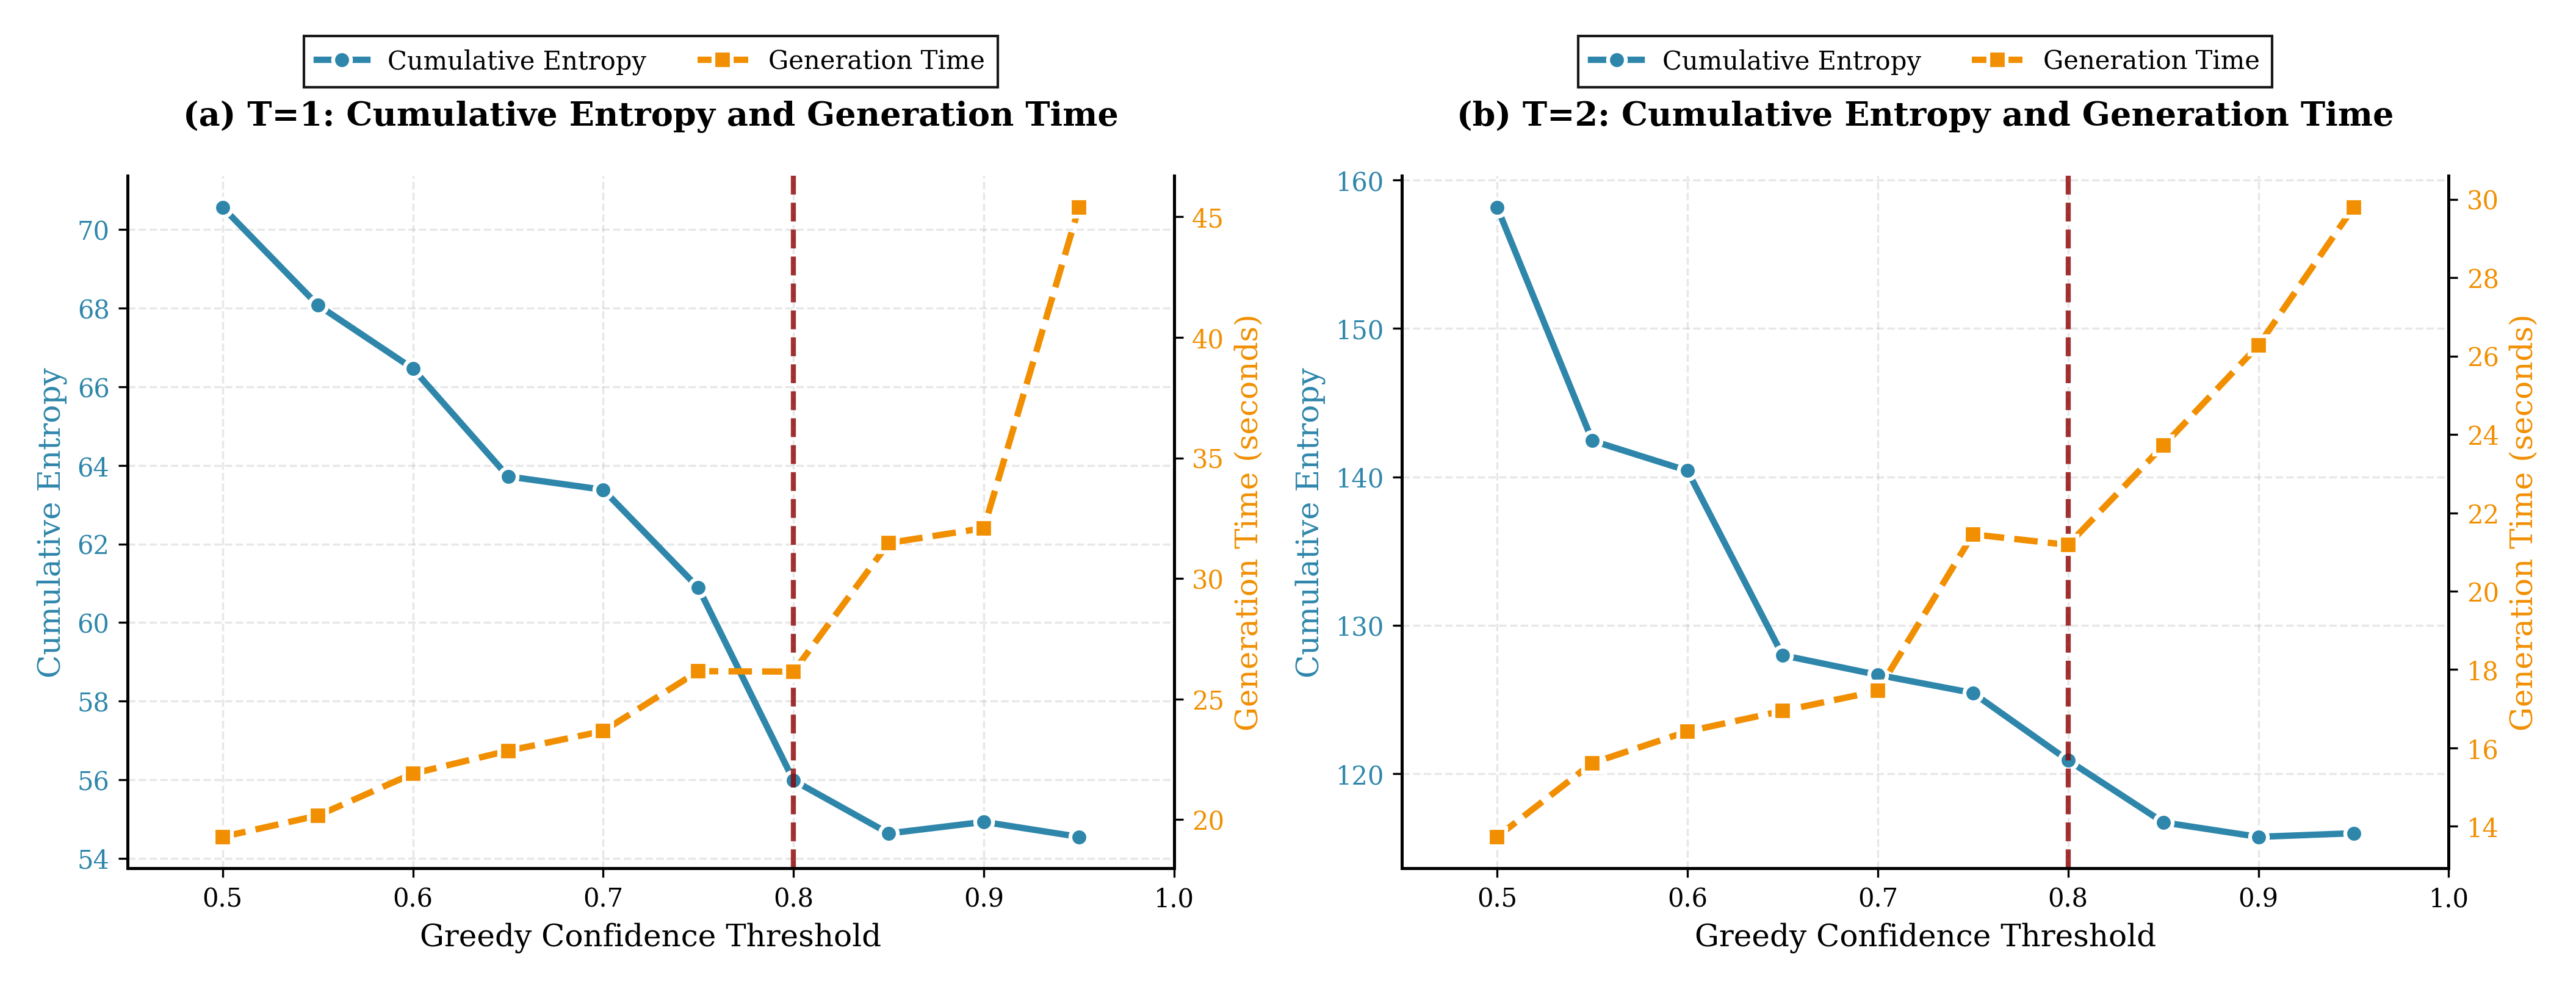
\includegraphics[width=0.9\linewidth]{abla-3.png}
    \caption{Effect of utility threshold on cumulative entropy reduction and generation time. }
    \label{fig:threshold_tradeoff}
\end{figure*}


\begin{figure*}[h]
    \centering
    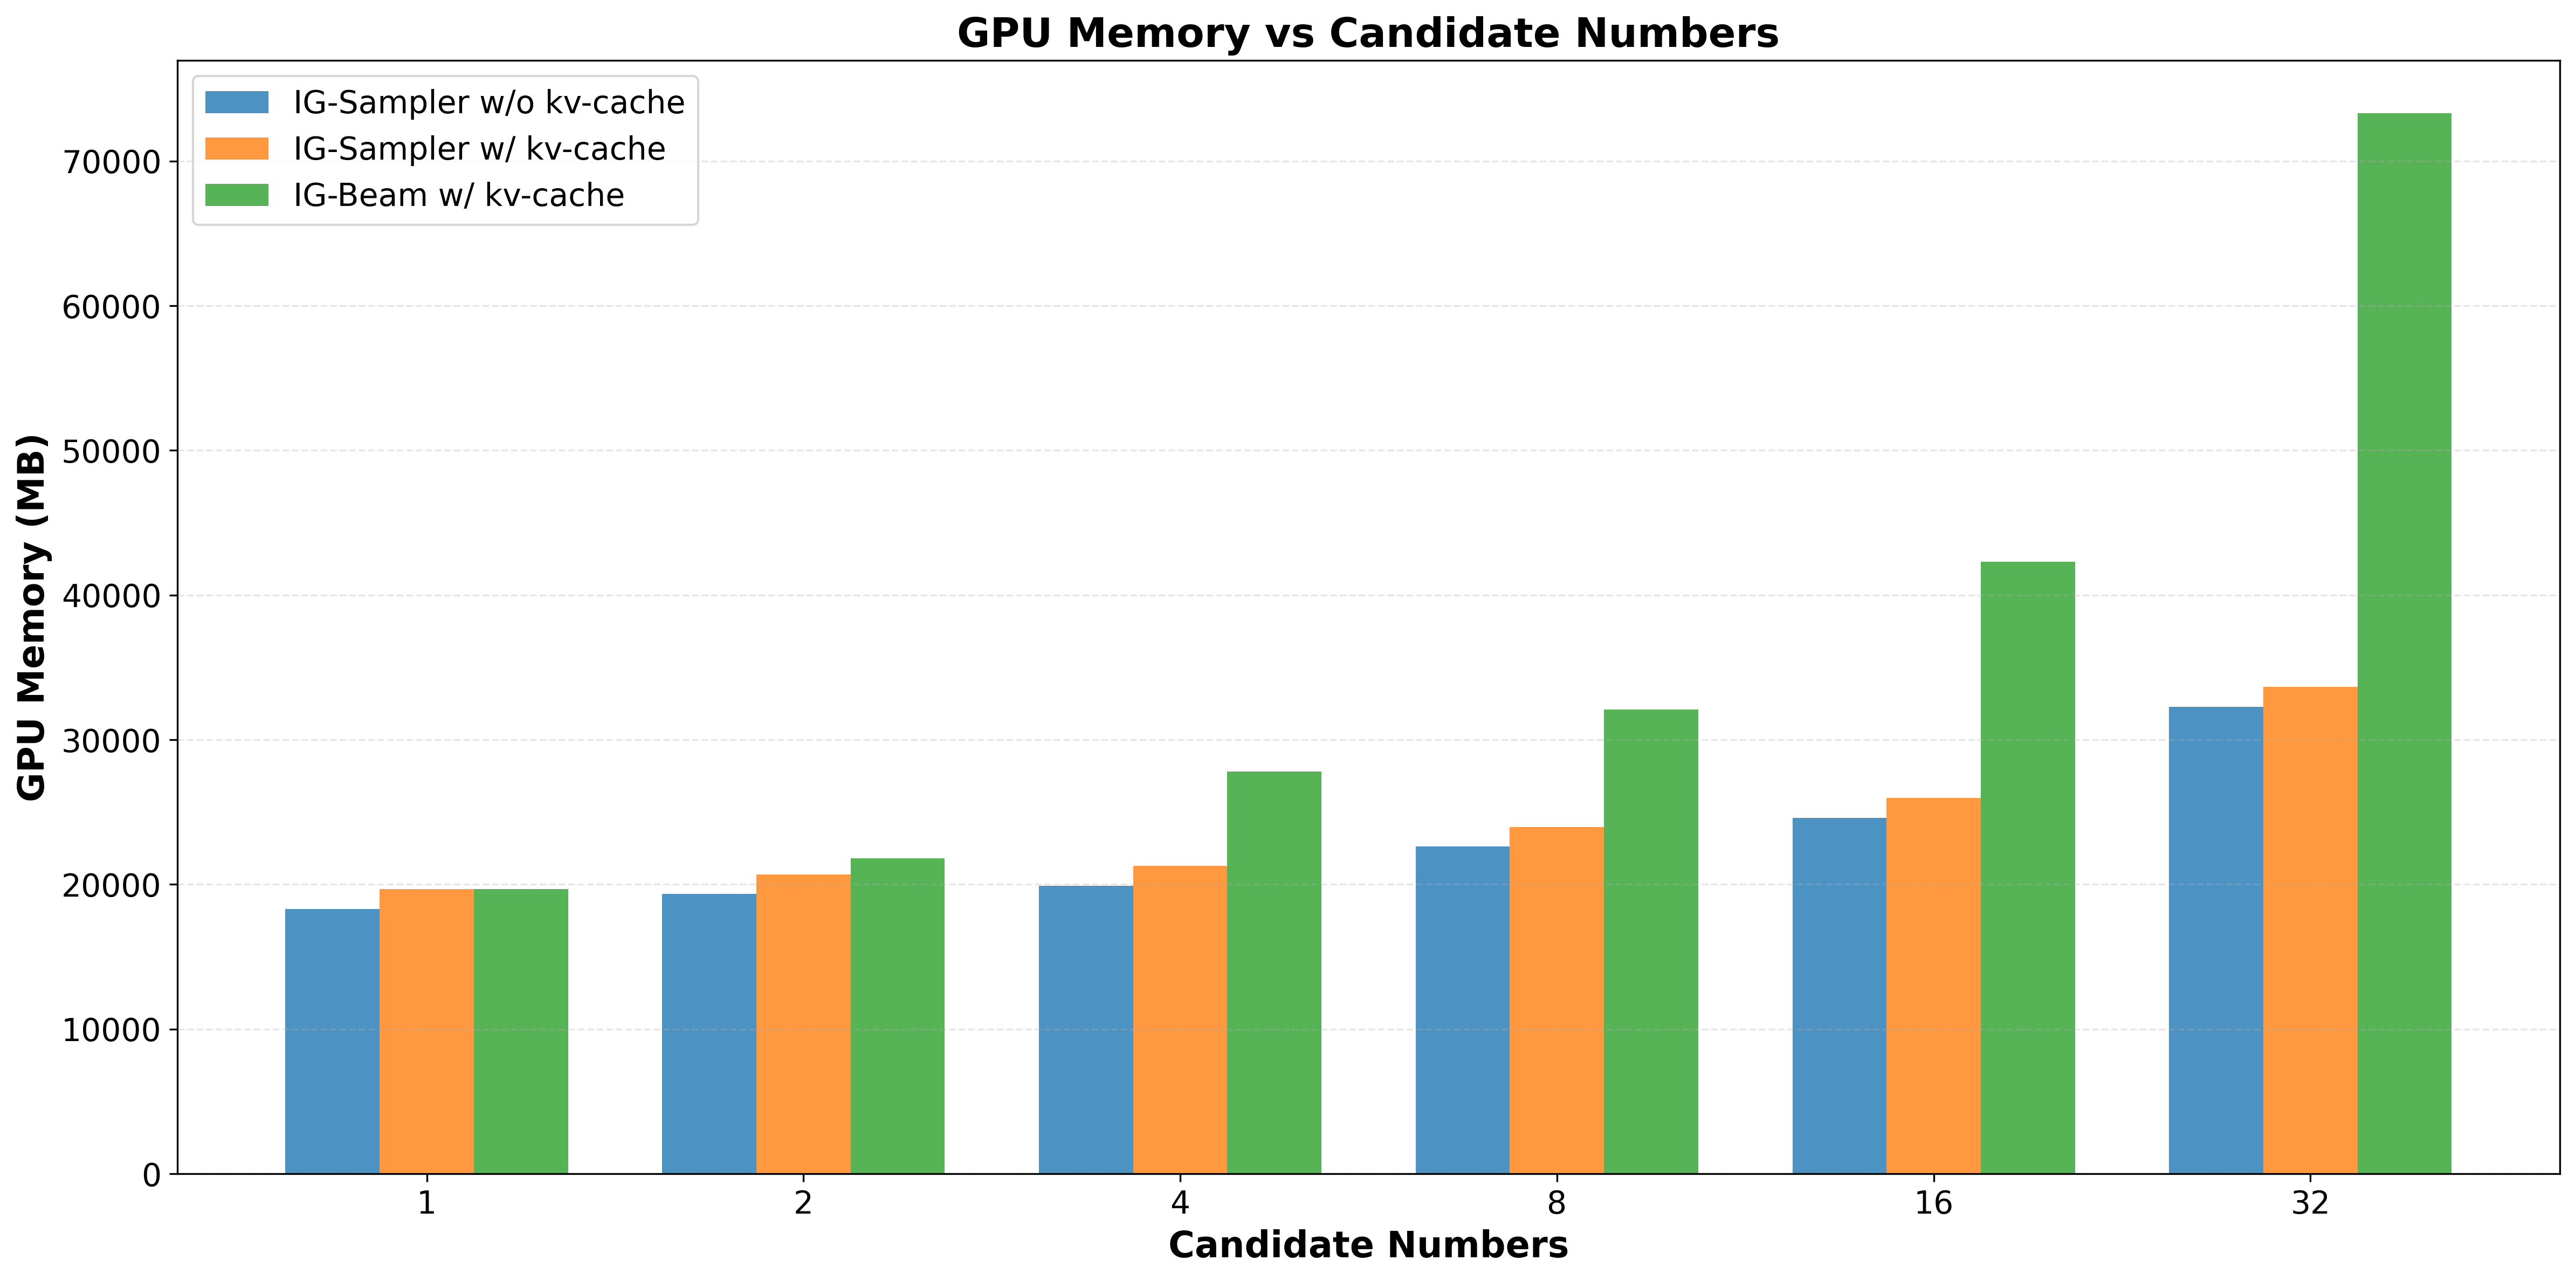
\includegraphics[width=0.8\linewidth]{gpu-compare.png}
    \caption{Memory usage comparison. Info-Gain Sampler maintains low overhead via prefix sharing.}
    \label{fig:gpu-compare}
\end{figure*}

